\documentclass[11pt]{article}
\usepackage[margin=1in]{geometry}
\usepackage{amsmath,amssymb}
\usepackage{graphicx}
\usepackage{booktabs}
\usepackage{multirow}
\usepackage[numbers,sort&compress]{natbib}
\usepackage[hidelinks]{hyperref}
\usepackage{caption}

\graphicspath{{../astro_poster/}{../../../open-kbp-modified/openkbp_hn_robustness/figures/}}

\title{Assessing the Generalizability and Robustness of Deep-Learning Dose
Prediction in Head-and-Neck Radiotherapy to Clinically Realistic CT
Perturbations}

\author{
Neil Tripathi$^{1}$, Rahim Chowdhury$^{2}$, Lei Ren$^{3}$, Amit Sawant$^{3}$,
Birjoo Vaishnav$^{3}$\\[4pt]
\small $^{1}$Department of Computer Science, New York University, New York, NY\\
\small $^{2}$University of Maryland Medical System, St.\ Joseph Medical Center, Baltimore, MD\\
\small $^{3}$Department of Radiation Oncology, University of Maryland, School of Medicine, Baltimore, MD
}
\date{Draft of \today}

\begin{document}
\maketitle

\begin{abstract}
\noindent\textbf{Purpose:} Deep-learning dose prediction models are
increasingly deployed across institutions, where they encounter computed
tomography (CT) images acquired on different scanners, with different
reconstruction kernels, dose levels, and artifact content. In contrast to
worst-case adversarial perturbations, these represent benign, physically
plausible sources of input variability. This study quantifies the robustness
of a head-and-neck dose prediction model to five families of clinically
realistic CT perturbations and identifies the image-quality factors that
materially affect predicted dose.

\noindent\textbf{Methods:} A 3D U-Net dose predictor with
squeeze-and-excitation attention (baseline dose score 3.73~Gy, DVH score
2.53~Gy on the OpenKBP benchmark) was evaluated on 40 held-out test patients
under 26 CT input conditions: an unperturbed baseline and five perturbation
families, each applied at five severity levels. The families model
acquisition noise, Hounsfield-unit (HU) calibration shift, low-frequency bias
field, spatial-resolution loss, and dental streak artifact, with severity
ranges chosen to meet or exceed American College of Radiology (ACR)
CT-simulation quality-assurance limits. Perturbations were applied to the
model input CT only; structure sets were held fixed, and each perturbed
prediction was compared with the same patient's unperturbed prediction. A
perturbation level was defined as clinically visible when the cohort-mean
change in any of 23 dose-volume histogram (DVH) criteria exceeded 1.0~Gy.

\noindent\textbf{Results:} Four of the five families produced no clinically
visible change at any tested severity, including severities well beyond
clinical plausibility. Spatial-resolution loss was the only family to cross
the threshold: the larynx near-maximum dose (D$_{0.1\mathrm{cc}}$) exceeded
1.0~Gy at a 2.0/1.0-voxel anisotropic blur, a level within realistic
cross-scanner variation in slice thickness and reconstruction kernel, and
reached 2.84~Gy (an 18.2\% DVH-score degradation) at the highest severity.
Bone-weighted HU calibration shift produced a measurable but sub-threshold
effect only at an implausible 1000~HU offset (0.61~Gy). Acquisition noise,
bias field, and dental streaks never exceeded 0.34~Gy on any criterion.

\noindent\textbf{Conclusions:} The model is robust to intensity-based CT
variability but systematically sensitive to spatial-resolution degradation,
which becomes clinically visible within the range of realistic inter-scanner
variation. Multi-institution quality assurance for learned dose prediction
should prioritize CT spatial-resolution and reconstruction-kernel
consistency over intensity calibration, and dose-based rather than
image-quality metrics should be used to assess the suitability of CBCT and
synthetic CT inputs.
\end{abstract}

\section{Introduction}

Deep-learning dose prediction is increasingly used to support automated,
knowledge-based, and adaptive radiotherapy treatment planning
\citep{babier2021openkbp}. A model trained at one institution must generalize
to CT images acquired under different conditions: scanner hardware,
reconstruction kernel, tube current, slice thickness, and patient-specific
artifacts all vary across and within clinics. Evaluation of these models,
however, is typically limited to prediction accuracy on a held-out test set
drawn from the same distribution as the training data. Consequently, model
robustness to realistic input variability remains poorly characterized, and
accuracy-based assessments may overlook failure modes that affect clinically
relevant outputs.

Prior work, including our own, has probed the sensitivity of dose prediction
networks with adversarial perturbations such as the fast gradient sign method
(FGSM) and projected gradient descent (PGD) \citep{goodfellow2015fgsm}. Such
attacks establish worst-case bounds but answer a different question from the
one facing a clinic that deploys a trained model on a new scanner: adversarial
perturbations are optimized against the model, whereas real-world image
variability is benign, structured, and physically constrained. A model may be
fragile under adversarial attack yet perfectly stable under any input change
that can actually occur in practice, or vice versa.

This study addresses the deployment question directly. We construct five
families of physically motivated CT perturbations, each a controlled model of
one real-world source of image variability: quantum acquisition noise,
scanner HU calibration drift, low-frequency intensity inhomogeneity, loss of
spatial resolution, and dental metal streak artifact. Each family is applied
over a five-level severity sweep spanning routine clinical variation, ACR
CT-simulation quality-assurance tolerances, and deliberately supra-clinical
extremes. We then determine, per family, the severity at which the perturbation
first produces a clinically significant change in predicted dose. The result is
a ranking of CT image-quality factors by their relevance to the safe
multi-institution deployment of a learned dose predictor.

\section{Methods}

\subsection{Dataset}

All experiments use the OpenKBP head-and-neck cohort
\citep{babier2021openkbp}, a public benchmark of 340 oropharyngeal cancer
patients planned for intensity-modulated radiotherapy with prescriptions of
70, 63, and 56~Gy delivered in 35 fractions. Each patient comprises a CT
volume and binary masks for up to ten regions of interest: seven organs at
risk (brainstem, spinal cord, right and left parotid glands, esophagus,
larynx, mandible) and three planning target volumes (PTV56, PTV63, PTV70).
All volumes are provided on a $128 \times 128 \times 128$ voxel grid with
approximately $3.9 \times 3.9 \times 2.5$~mm$^3$ voxels. We use the standard
partition of 200 training and 40 held-out test patients; all robustness
results are reported on the 40 test patients. CT intensities are stored as
non-negative values offset such that air is near 0 and water near 1024
(true HU plus 1024), clipped to $[0, 4095]$, and normalized to $[0,1]$ for
network input. Dose is normalized by the 70~Gy prescription.

\subsection{Dose prediction model}

The predictor is a 3D U-Net \citep{ronneberger2015unet} with six encoder
stages (64 to 512 filters) and five decoder stages with skip connections.
Instance normalization is used throughout, residual connections are included
within encoder and decoder blocks, and squeeze-and-excitation channel
attention \citep{hu2018squeeze} is applied at the deepest levels. The network
receives the CT volume and the ten structure masks and outputs a voxel-wise
3D dose distribution. It was trained for 100 epochs with a masked mean
absolute error loss restricted to the feasible dose region, a $4\times$
loss weighting on PTV voxels, mixed-precision arithmetic, and flip and
intensity-scaling augmentation. On the OpenKBP test set the model achieves a
dose score (voxel-wise mean absolute dose error within the feasible region)
of 3.73~Gy and a DVH score (mean absolute error over the standard OpenKBP DVH
criteria) of 2.53~Gy, compared with 2.43 and 1.48~Gy for the competition-winning
ensemble. The model is used exactly as trained; no fine-tuning, test-time
adaptation, or perturbation-aware augmentation is applied in this study.

\subsection{Perturbation families}
\label{sec:families}

Each family perturbs the CT volume only, inside the patient body mask, with
all outputs clipped back to the valid intensity range $[1, 4095]$. Structure
masks are never modified. Randomness is controlled by a deterministic seed
derived from the (family, level, patient) triple, making the entire perturbed
dataset exactly reproducible. Severity parameters for all levels are listed in
Table~\ref{tab:severity}.

\paragraph{P1: Signal-dependent acquisition noise.} Zero-mean Gaussian noise
with a per-voxel standard deviation that is larger in bone than in soft
tissue, modeling the heteroscedastic quantum noise of CT detectors:
\begin{equation}
\tilde{x}(v) = x(v) + \varepsilon(v), \qquad
\varepsilon(v) \sim \mathcal{N}\!\left(0, \sigma(v)^2\right), \qquad
\sigma(v) = \begin{cases} \sigma_\mathrm{bone} & x(v) > 1500 \\
\sigma_\mathrm{soft} & \text{otherwise,} \end{cases}
\end{equation}
with $(\sigma_\mathrm{soft}, \sigma_\mathrm{bone})$ swept from $(8, 12)$ to
$(100, 160)$~HU. Typical single-scanner noise is approximately 10 to 50~HU,
so the upper levels substantially exceed clinical reality.

\paragraph{P2: Bone-weighted HU calibration shift.} A systematic intensity
offset with random sign, interpolated smoothly between a soft-tissue value
and a larger bone value through a sigmoid gate centered at 1500 stored HU
with width 200:
\begin{equation}
\tilde{x}(v) = x(v) + s\left[\Delta_\mathrm{soft} +
(\Delta_\mathrm{bone} - \Delta_\mathrm{soft})\,
\sigma\!\left(\tfrac{x(v) - 1500}{200}\right)\right],
\qquad s \in \{-1, +1\},
\end{equation}
modeling calibration drift and cross-scanner HU differences, which are
typically 10 to 50~HU in soft tissue. The sweep extends to a deliberately
implausible $(100, 1000)$~HU offset.

\paragraph{P3: Low-frequency bias field.} A smooth multiplicative-style
shading field added within the body, constructed as the sum of three
separable 3D cosine harmonics with random frequencies (0.5 to 2.5 cycles per
field of view), phases, and weights, normalized to unit peak and scaled to an
amplitude swept from 10 to 200~HU. This models scatter- or
calibration-induced spatial nonuniformity, which is realistically tens of HU.

\paragraph{P4: Spatial-resolution loss.} Anisotropic Gaussian blur with
through-slice standard deviation $\sigma_z$ twice the in-plane
$\sigma_{xy}$, modeling thicker slice acquisition and smoother reconstruction
kernels:
\begin{equation}
\tilde{x} = G_{(\sigma_z, \sigma_{xy}, \sigma_{xy})} * x,
\end{equation}
with $(\sigma_z, \sigma_{xy})$ swept from $(0.5, 0.25)$ to $(4.0, 2.0)$
voxels (levels L0 to L4). Realistic cross-scanner variation in slice
thickness and kernel corresponds to roughly 1 to 3 voxels of effective blur
on this grid.

\paragraph{P5: Dental streak artifact.} A radial pattern of alternating
bright and dark streaks anchored at the mandible centroid, with Gaussian
angular profiles, radial decay (40-voxel length constant), Gaussian
through-slice decay (3-slice standard deviation), and a saturated metal spot
(3-voxel radius) at the centroid. Amplitude and streak count are swept from
(150~HU, 8 streaks) to (1200~HU, 24 streaks). Dental artifacts of this
character are common in head-and-neck CT.

\subsection{Evaluation protocol}

The 26 conditions (baseline plus five families at five levels each) define 26
versions of the 40-patient test set, 1040 model inferences in total. For each
condition the model re-predicts dose from the perturbed CT with the original
structure masks. Impact is quantified against each patient's own unperturbed
prediction, isolating the causal effect of the image perturbation from
baseline model error. Two metric groups are computed:

\begin{itemize}
\item \textbf{Voxel-wise:} mean absolute dose difference (MAE, Gy) within the
feasible dose region, aggregated as the OpenKBP dose score; and the fraction
of patients whose MAE change exceeds 0.5~Gy.
\item \textbf{DVH criteria:} the 23 standard OpenKBP criteria, namely
D$_{0.1\mathrm{cc}}$ and mean dose for each organ at risk, and D$_{99}$,
D$_{95}$, and D$_{1}$ for each target, aggregated as the OpenKBP DVH score
and also examined per criterion.
\end{itemize}

\paragraph{Clinical visibility threshold.} A severity level is defined as
\emph{clinically visible} when the cohort-mean absolute change in \emph{any
single} DVH criterion, relative to each patient's unperturbed prediction,
exceeds 1.0~Gy. The per-criterion definition is deliberately more sensitive
than a threshold on the aggregate DVH score, which averages over 23 criteria
and can mask a large error confined to one structure. The fraction of
patients with MAE change above 0.5~Gy is reported as a corroborating metric
but is not part of the gate.

\section{Results}

\subsection{Aggregate degradation}

Table~\ref{tab:aggregate} reports the dose score and DVH score for all 26
conditions. Four families are essentially flat across their full sweeps: the
largest aggregate DVH-score change is $+1.43\%$ for acquisition noise at
$(100, 160)$~HU, $+0.42\%$ for the bias field at 200~HU, and $+0.87\%$ for
dental streaks at 1200~HU, all at severities well beyond clinical ranges.
The HU calibration shift is flat through L3 and becomes measurable only at
the implausible extremes, reaching $+11.2\%$ DVH score at a 1000~HU bone
offset. Spatial-resolution loss is the clear outlier: degradation grows
approximately linearly with blur, from $+1.5\%$ DVH score at near-native
resolution (L0) to $+18.2\%$ at L4, with the dose score rising from 3.73 to
4.12~Gy.

\begin{table}[t]
\centering
\caption{Severity parameters for the five perturbation families. P4 uses
levels L0 to L4; all other families use L1 to L5.}
\label{tab:severity}
\small
\begin{tabular}{llccccc}
\toprule
Family & Parameter (units) & \multicolumn{5}{c}{Level} \\
\cmidrule(lr){3-7}
 & & 1 & 2 & 3 & 4 & 5 \\
\midrule
P1 noise & $\sigma_\mathrm{soft}/\sigma_\mathrm{bone}$ (HU) & 8/12 & 15/25 & 30/50 & 60/100 & 100/160 \\
P2 HU shift & $\Delta_\mathrm{soft}/\Delta_\mathrm{bone}$ (HU) & 5/50 & 10/100 & 25/250 & 50/500 & 100/1000 \\
P3 bias field & amplitude (HU) & 10 & 20 & 50 & 100 & 200 \\
P4 resolution & $\sigma_z/\sigma_{xy}$ (voxels) & 0.5/0.25 & 1.0/0.5 & 2.0/1.0 & 3.0/1.5 & 4.0/2.0 \\
P5 dental & amplitude (HU) / streaks & 150/8 & 300/12 & 500/16 & 800/20 & 1200/24 \\
\bottomrule
\end{tabular}
\end{table}

\begin{table}[t]
\centering
\caption{Dose score (voxel-wise MAE, Gy) and DVH score (Gy) for all 26
conditions, 40 test patients. Deltas are relative to the unperturbed
baseline.}
\label{tab:aggregate}
\small
\begin{tabular}{llcccc}
\toprule
Family & Level & Dose score (Gy) & DVH score (Gy) & $\Delta$DVH (Gy) & $\Delta$DVH (\%) \\
\midrule
Baseline & -- & 3.731 & 2.535 & -- & -- \\
\midrule
\multirow{5}{*}{P1 noise}
 & L1 & 3.731 & 2.535 & 0.000 & 0.01 \\
 & L2 & 3.733 & 2.538 & 0.003 & 0.13 \\
 & L3 & 3.737 & 2.543 & 0.009 & 0.34 \\
 & L4 & 3.742 & 2.559 & 0.024 & 0.96 \\
 & L5 & 3.742 & 2.571 & 0.036 & 1.43 \\
\midrule
\multirow{5}{*}{P2 HU shift}
 & L1 & 3.730 & 2.531 & $-0.004$ & $-0.15$ \\
 & L2 & 3.740 & 2.544 & 0.010 & 0.38 \\
 & L3 & 3.751 & 2.519 & $-0.016$ & $-0.61$ \\
 & L4 & 3.793 & 2.572 & 0.037 & 1.46 \\
 & L5 & 3.916 & 2.818 & 0.284 & 11.19 \\
\midrule
\multirow{5}{*}{P3 bias field}
 & L1 & 3.732 & 2.535 & 0.000 & 0.01 \\
 & L2 & 3.730 & 2.534 & $-0.001$ & $-0.04$ \\
 & L3 & 3.736 & 2.534 & $-0.000$ & $-0.01$ \\
 & L4 & 3.733 & 2.524 & $-0.011$ & $-0.44$ \\
 & L5 & 3.759 & 2.545 & 0.011 & 0.42 \\
\midrule
\multirow{5}{*}{P4 resolution}
 & L0 & 3.739 & 2.573 & 0.038 & 1.50 \\
 & L1 & 3.780 & 2.636 & 0.101 & 4.00 \\
 & L2 & 3.885 & 2.729 & 0.194 & 7.67 \\
 & L3 & 3.982 & 2.824 & 0.289 & 11.40 \\
 & L4 & 4.124 & 2.995 & 0.460 & 18.15 \\
\midrule
\multirow{5}{*}{P5 dental}
 & L1 & 3.729 & 2.541 & 0.007 & 0.26 \\
 & L2 & 3.730 & 2.545 & 0.011 & 0.42 \\
 & L3 & 3.730 & 2.552 & 0.017 & 0.67 \\
 & L4 & 3.731 & 2.557 & 0.022 & 0.87 \\
 & L5 & 3.732 & 2.555 & 0.021 & 0.82 \\
\bottomrule
\end{tabular}
\end{table}

\subsection{Per-criterion threshold analysis}

The clinical-visibility analysis examines the worst single DVH criterion per
condition (Table~\ref{tab:threshold}). Spatial-resolution loss is the only
family that crosses the 1.0~Gy threshold anywhere in the tested range. The
sentinel criterion is the larynx near-maximum dose (D$_{0.1\mathrm{cc}}$),
which shifts by 0.22~Gy at L0, 0.59~Gy at L1, 1.15~Gy at L2 (the first
crossing), 1.68~Gy at L3, and 2.84~Gy at L4. At L4 a second criterion also
exceeds 1~Gy. The corroborating voxel-wise metric follows the same pattern:
the fraction of patients with an MAE change above 0.5~Gy grows from 0.00 at
L0--L1 to 0.05, 0.12, and 0.23 at L2, L3, and L4.

No other family reaches the threshold on any criterion at any severity. The
HU calibration shift peaks at 0.61~Gy (PTV56 D$_1$) at the 1000~HU offset;
acquisition noise peaks at 0.14~Gy (spinal cord D$_{0.1\mathrm{cc}}$); the
bias field at 0.09~Gy (right parotid mean); and dental streaks at 0.33~Gy
(PTV70 D$_1$).

\begin{table}[t]
\centering
\caption{Worst single-criterion DVH shift (cohort mean, Gy) per family, the
sentinel criterion, the number of criteria exceeding 1.0~Gy, and the fraction
of patients whose voxel-wise MAE rises by more than 0.5~Gy.}
\label{tab:threshold}
\small
\begin{tabular}{lcccc}
\toprule
Condition & Max shift (Gy) & Sentinel criterion & \#\,$>1$~Gy & Frac.\ MAE$>0.5$~Gy \\
\midrule
P1 noise, L5 (worst) & 0.14 & Spinal cord D$_{0.1\mathrm{cc}}$ & 0 & 0.00 \\
P2 HU shift, L4 & 0.41 & Larynx D$_{0.1\mathrm{cc}}$ & 0 & 0.03 \\
P2 HU shift, L5 & 0.61 & PTV56 D$_1$ & 0 & 0.17 \\
P3 bias field (worst) & 0.09 & Right parotid mean & 0 & 0.00 \\
P4 resolution, L0 & 0.22 & Larynx D$_{0.1\mathrm{cc}}$ & 0 & 0.00 \\
P4 resolution, L1 & 0.59 & Larynx D$_{0.1\mathrm{cc}}$ & 0 & 0.00 \\
\textbf{P4 resolution, L2} & \textbf{1.15} & Larynx D$_{0.1\mathrm{cc}}$ & 1 & 0.05 \\
\textbf{P4 resolution, L3} & \textbf{1.68} & Larynx D$_{0.1\mathrm{cc}}$ & 1 & 0.12 \\
\textbf{P4 resolution, L4} & \textbf{2.84} & Larynx D$_{0.1\mathrm{cc}}$ & 2 & 0.23 \\
P5 dental (worst) & 0.33 & PTV70 D$_1$ & 0 & 0.00 \\
\bottomrule
\end{tabular}
\end{table}

\subsection{Spatial and structural error patterns}

Example perturbed CT slices and the corresponding dose-difference maps are
shown in Figures~\ref{fig:ct} and \ref{fig:dose}. The four intensity families
alter voxel values while leaving anatomical boundaries intact, and their
dose-difference maps are near zero and spatially unstructured. Resolution
loss visibly erodes tissue boundaries, and its dose errors are spatially
structured, concentrating at structure boundaries and in the dose-gradient
regions between targets and adjacent organs at risk. Per-structure analysis
at the highest severity shows the largest relative error inflation in
geometrically complex, boundary-dependent structures: the larynx, the parotid
glands, and the mandible. The severity progression for resolution loss
(Figure~\ref{fig:threshold}) shows the approximately linear growth of the
worst-criterion shift with blur and the crossing of the 1.0~Gy line between
L1 and L2.

\begin{figure}[t]
\centering
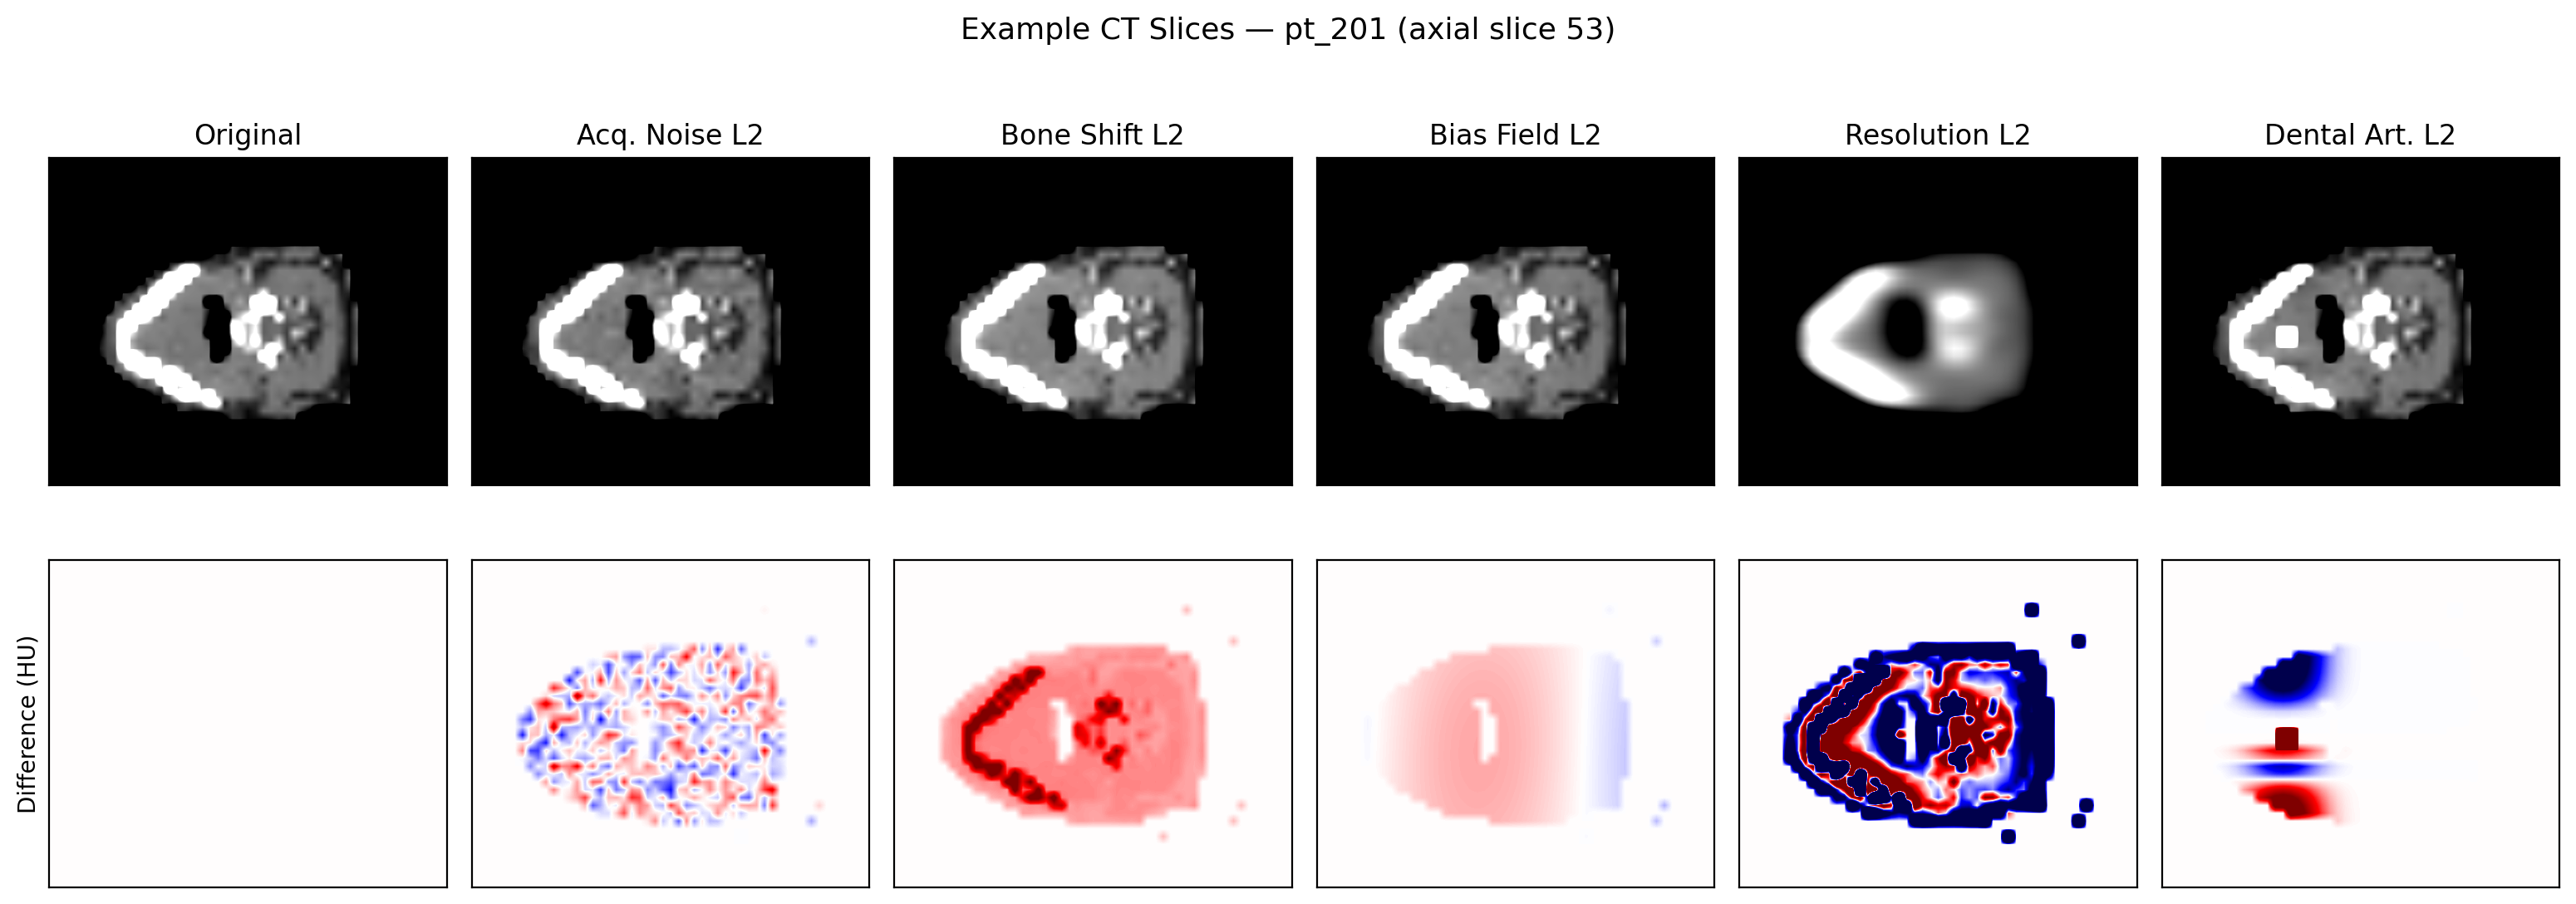
\includegraphics[width=\textwidth]{ct_slices_axial.png}
\caption{Axial CT slice (patient pt\_201) unperturbed and under each
perturbation family at an intermediate severity (top), with HU difference
maps (bottom). Intensity families preserve anatomical boundaries; resolution
loss erodes them.}
\label{fig:ct}
\end{figure}

\begin{figure}[t]
\centering
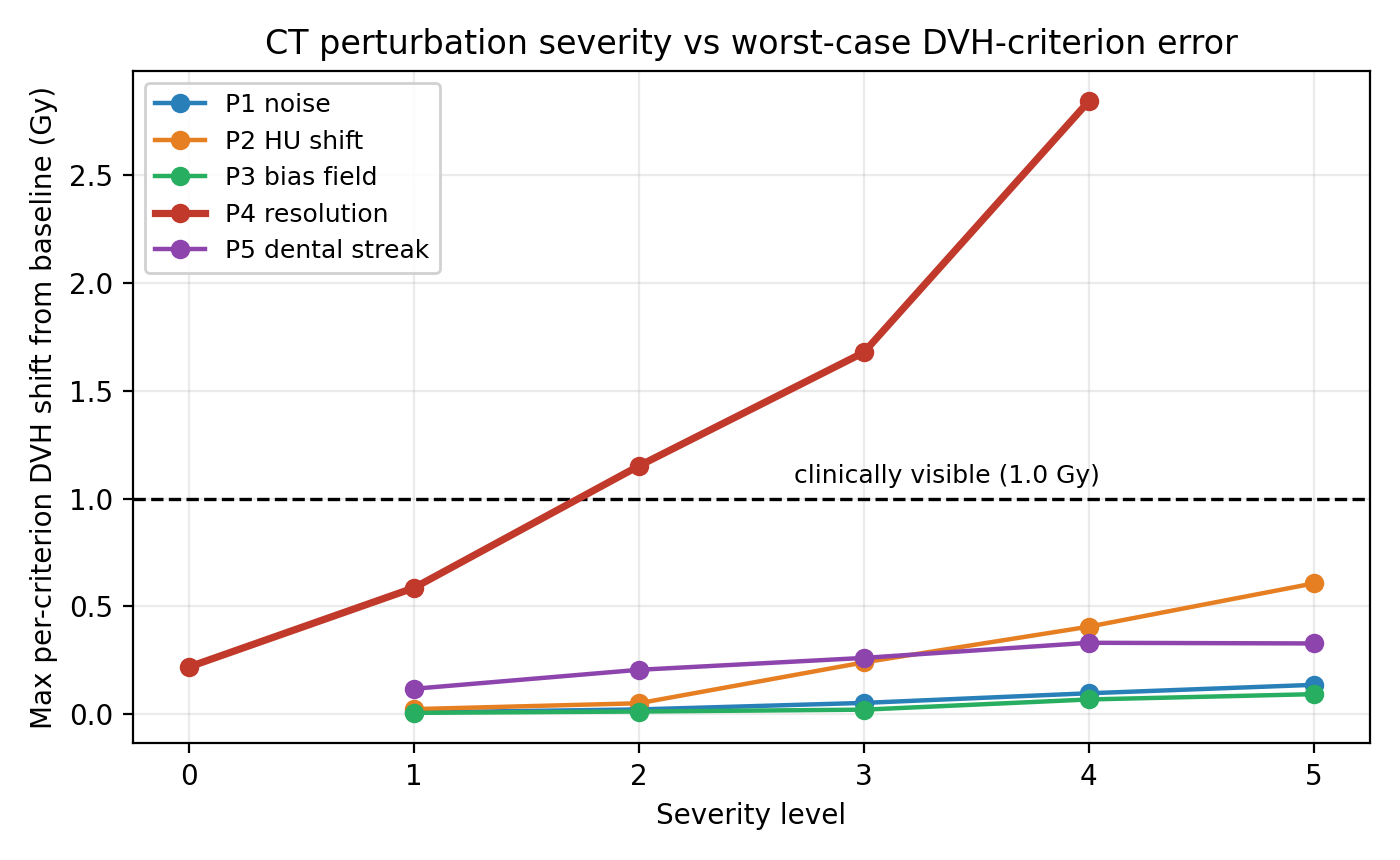
\includegraphics[width=\textwidth]{fig_panel5_maxcrit_gy.png}
\caption{Worst single-criterion DVH shift (cohort mean, Gy) versus severity
level for the five families. The dashed line marks the 1.0~Gy clinical
visibility threshold. Only spatial-resolution loss (P4) crosses it, between
L1 and L2.}
\label{fig:threshold}
\end{figure}

\begin{figure}[t]
\centering
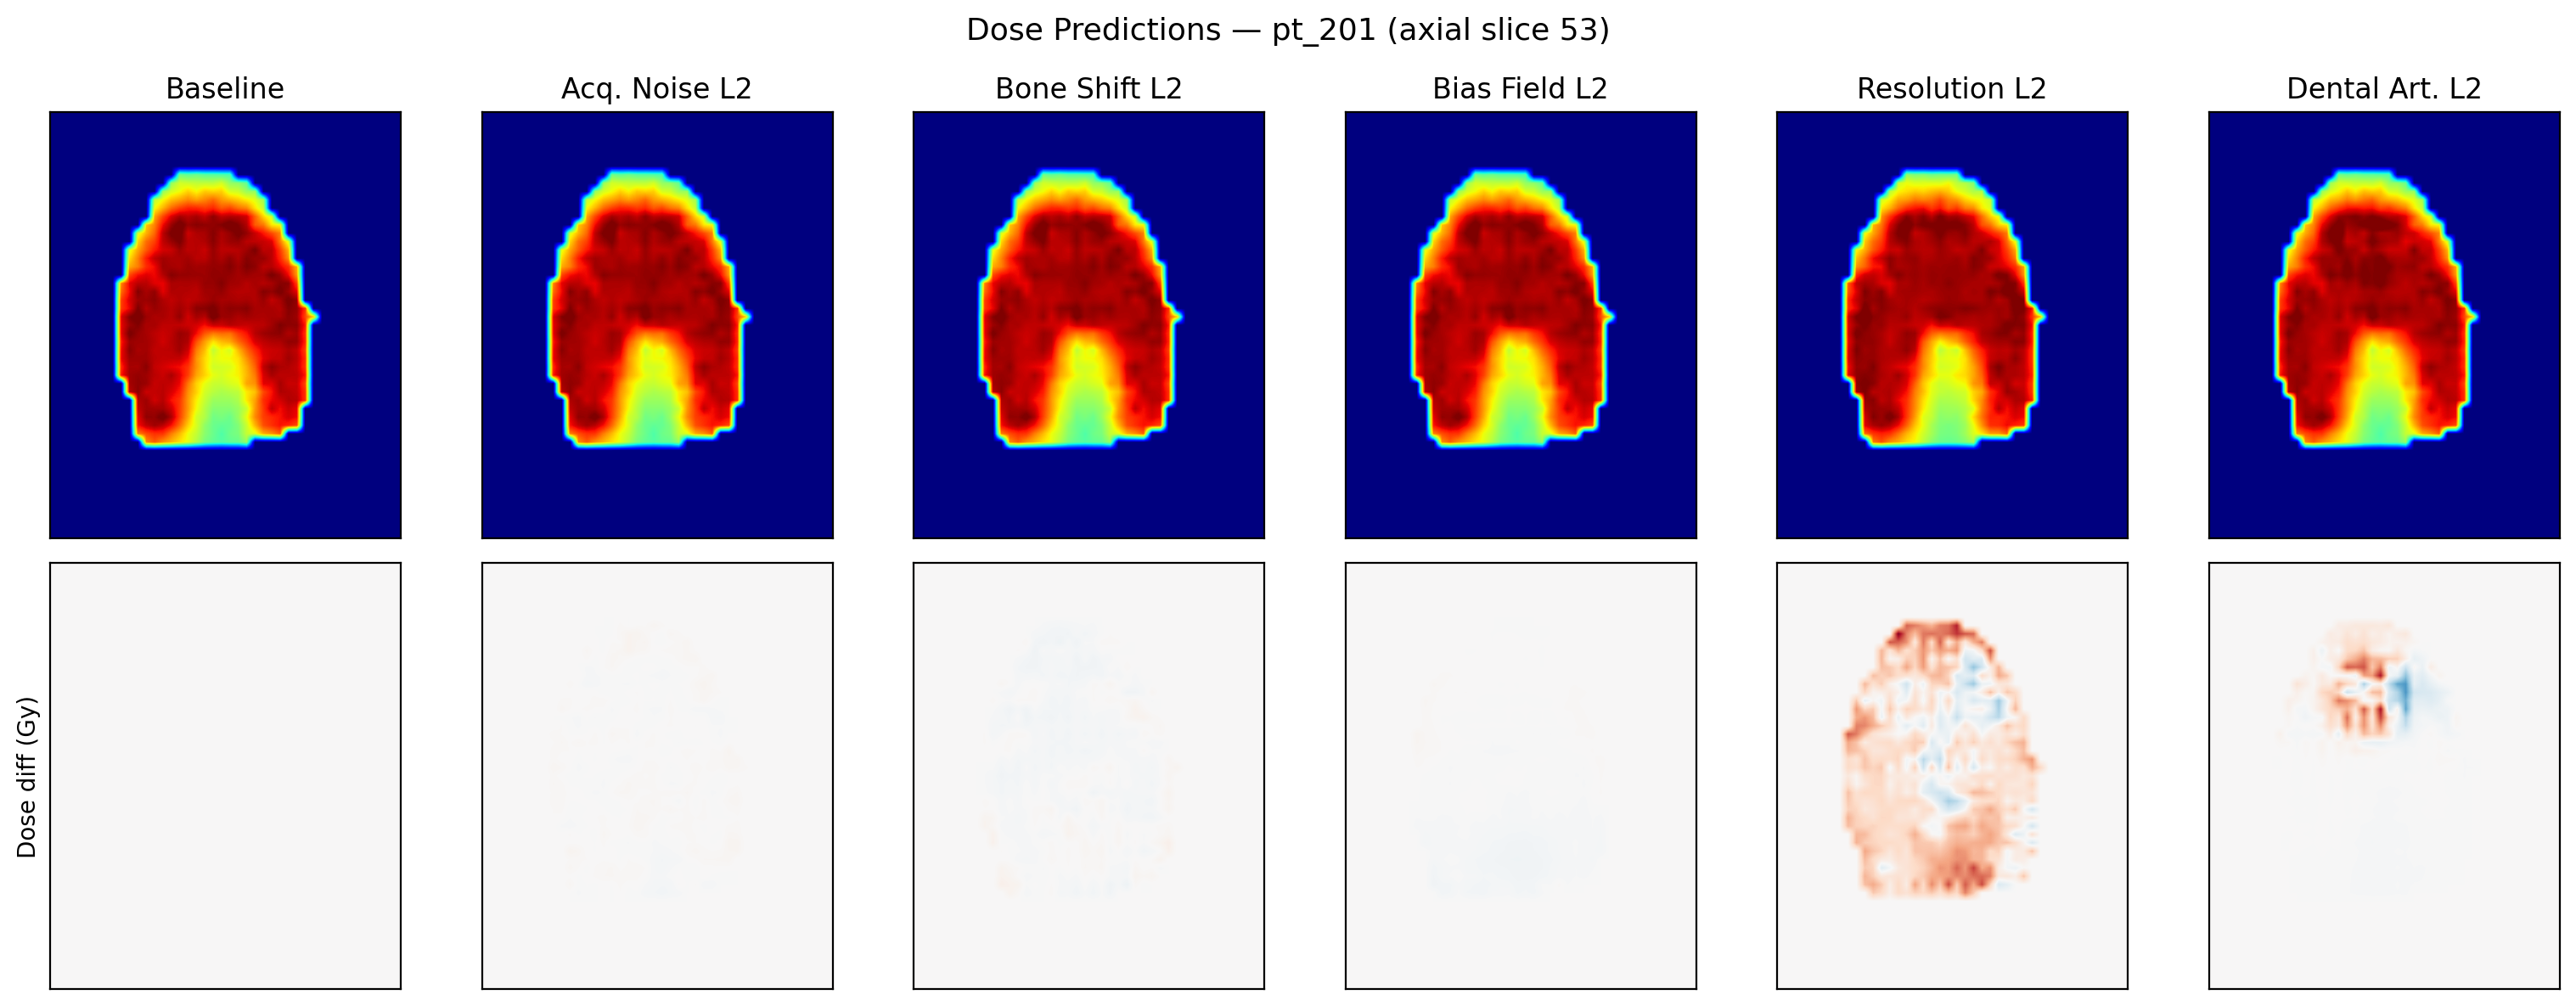
\includegraphics[width=\textwidth]{dose_difference_axial.png}
\caption{Predicted dose (top) and difference from the unperturbed prediction
(bottom) for each family at an intermediate severity. Resolution loss
produces spatially structured errors at anatomical boundaries; the other
families are near zero.}
\label{fig:dose}
\end{figure}

\section{Discussion}

The central finding is a sharp asymmetry between intensity-based and
geometry-based input variability. The model tolerates intensity perturbations
at severities far beyond clinical plausibility: noise at $2\times$ to
$3\times$ typical scanner levels, calibration offsets an order of magnitude
above realistic drift, shading fields of 200~HU, and dense high-amplitude
streak artifacts all leave every DVH criterion within 1~Gy of the unperturbed
prediction. A plausible mechanism is that these perturbations preserve the
structural boundaries that the network, which also receives the structure
masks as input, uses to localize dose gradients; zero-mean or slowly varying
intensity changes are largely averaged out by the convolutional feature
hierarchy.

Spatial-resolution loss breaks exactly this invariance. Blur removes the
high-frequency boundary information on which sharp dose gradients are
conditioned, and the resulting errors are spatially structured, appearing
first at the interfaces of small, geometrically complex structures. The
sentinel criterion, larynx near-maximum dose, is a near-maximum metric in a
small organ embedded between the pharyngeal target volumes, which is
precisely where boundary localization matters most. Importantly, the first
threshold crossing occurs at a 2.0/1.0-voxel blur, corresponding to roughly
5~mm through-slice and 4~mm in-plane full-width-at-half-maximum smoothing on
this grid, which is within the realistic range of cross-scanner slice
thickness and reconstruction-kernel differences. Resolution mismatch is
therefore not a tail risk but an expected condition of multi-institution
deployment.

These results complement adversarial robustness analyses. Our earlier
adversarial evaluation of the same class of models showed that optimized
perturbations far smaller than any of the levels used here can produce large
dosimetric errors. The present study shows that among perturbations that
actually occur in practice, only resolution loss carries clinically relevant
risk for this model. The two analyses answer different questions: adversarial
attacks bound the worst case, whereas realistic perturbation sweeps rank the
operational risks. For deployment decisions the realistic ranking is the
actionable one, and it points at CT spatial-resolution consistency, not
intensity calibration, as the property to control.

Three practical implications follow. First, commissioning and ongoing quality
assurance for learned dose prediction should explicitly include a
resolution-mismatch test, for example by predicting on a resampled or
kernel-smoothed copy of a commissioning CT and verifying DVH stability.
Second, image-quality metrics tuned to intensity fidelity (noise, uniformity,
HU accuracy) are insufficient proxies for model safety; dose-based
end-to-end checks are required, particularly when considering CBCT or
synthetic CT inputs whose principal defects include resolution and boundary
degradation. Third, the approximately linear severity response of the
resolution family suggests that training-time blur augmentation may flatten
the curve, which is directly testable.

\subsection{Limitations}

This is a single-model, single-anatomy study on a public benchmark; the
threshold levels reported are specific to this network, training recipe, and
voxel grid, and the generality of the resolution failure mode across
architectures remains to be established (see Section~\ref{sec:future}).
Structure masks were held fixed under perturbation, isolating the image
pathway; in clinical reality, degraded images would also degrade contouring,
likely compounding the effect. The perturbation families are physically
motivated simulations rather than paired rescans, and the dental artifact
model is a geometric approximation of beam-hardening physics. The 1.0~Gy
per-criterion threshold, while grounded in the granularity of clinical plan
evaluation, is a choice; the full severity curves are reported so that any
alternative threshold can be applied. Finally, gamma analysis was not
computed; the evaluation is DVH- and voxel-MAE-based.

\section{Future work}
\label{sec:future}

Three extensions are planned. First, a multi-architecture comparison
deploying four to five distinct dose prediction models (a plain 3D U-Net, the
present SE U-Net, an attention or transformer-based variant such as Swin
UNETR, and a cascade or ensemble representative of the OpenKBP
state-of-the-art) under the identical 26-condition battery, to determine
whether the resolution sensitivity and its L2 crossing point are
architecture-specific or a property of the task. The perturbation and
evaluation pipeline is model-agnostic (CSV volumes in, CSV doses out), so
each additional model requires only 1040 inference passes. Second,
CBCT-characteristic degradations (scatter and cupping, ring artifacts, and
limited field-of-view truncation) to establish commissioning tolerances for
online adaptive radiotherapy. Third, distribution-free and certified
per-patient DVH prediction intervals under bounded CT perturbation, and
training-time resolution augmentation as a mitigation.

\section{Conclusions}

A head-and-neck deep-learning dose prediction model tolerates clinically
realistic intensity-based CT perturbations, including acquisition noise,
calibration drift, bias fields, and dental streak artifacts, at severities
meeting or exceeding ACR quality-assurance limits. It is systematically
sensitive to spatial-resolution degradation, which becomes clinically visible
(larynx D$_{0.1\mathrm{cc}}$ shift above 1~Gy) within the realistic range of
inter-scanner slice-thickness and reconstruction-kernel variation and grows
approximately linearly with blur. Multi-institution quality assurance for
learned dose prediction should prioritize CT spatial-resolution and
reconstruction-kernel consistency, and dose-based rather than image-quality
metrics should govern the acceptance of alternative image sources.

\bibliographystyle{unsrtnat}
\begin{thebibliography}{9}

\bibitem{babier2021openkbp}
Babier A, Mahon R, McNiven A, Diamant A, Chan TCY.
OpenKBP: The open-access knowledge-based planning grand challenge and dataset.
\emph{Med Phys}. 2021;48:4932--4948.

\bibitem{ronneberger2015unet}
Ronneberger O, Fischer P, Brox T.
U-Net: Convolutional networks for biomedical image segmentation.
\emph{MICCAI}. 2015;234--241.

\bibitem{hu2018squeeze}
Hu J, Shen L, Sun G.
Squeeze-and-excitation networks.
\emph{CVPR}. 2018;7132--7141.

\bibitem{goodfellow2015fgsm}
Goodfellow IJ, Shlens J, Szegedy C.
Explaining and harnessing adversarial examples.
\emph{ICLR}. 2015.

\bibitem{gao2025}
Gao Y, et al.
\emph{Phys Med Biol}. 2025;70:115006.

\bibitem{acr}
American College of Radiology.
CT quality control and accreditation guidelines.

\end{thebibliography}

\end{document}
